\documentclass[14pt, a4paper]{extarticle}

\usepackage{ProkhorovaGOST}
\usepackage{hyperref}
\usepackage{listings}
\usepackage{array}
\usepackage{caption}
\hypersetup{
	pdftex,
	colorlinks = true,
	linkcolor = black,
	filecolor = magenta,
	citecolor = green,      
	urlcolor = cyan,
}

% к таблице и листингу подпись сверху, перед каждым иллюстративным материалом анонсировать
% написатьт в квадратных скобках к рекурсии комментарием что это метод и понятно почему вызываем его снова
\definecolor{mylightgray}{RGB}{240,240,240}
\definecolor{mygreen}{rgb}{0,0.6,0}
\definecolor{mygray}{rgb}{0.5,0.5,0.5}
\definecolor{mymauve}{rgb}{0.58,0,0.82}

\lstset{
	backgroundcolor=\color{mylightgray},rulecolor=\color{red},  % choose the background color; you must add \usepackage{color} or \usepackage{xcolor}; should come as last argument
	basicstyle=\footnotesize\ttfamily,        % the size of the fonts that are used for the code
	breakatwhitespace=false,         % sets if automatic breaks should only happen at whitespace
	breaklines=true,                 % sets automatic line breaking
	captionpos=t,                    % sets the caption-position to bottom
	commentstyle=\color{mygreen},    % comment style
	extendedchars=false,              % lets you use non-ASCII characters; for 8-bits encodings only, does not work with UTF-8
	firstnumber=0,                % start line enumeration with line 1000
	frame=shadowbox,
	%rulesepcolor=\color{green},	                   % adds a frame around the code
	keepspaces=true,                 % keeps spaces in text, useful for keeping indentation of code (possibly needs columns=flexible)
	keywordstyle=\color{blue}\textbf,       % keyword style
	language=Python,                 % the language of the code
	morekeywords={*,...},            % if you want to add more keywords to the set
	numbers=left,                    % where to put the line-numbers; possible values are (none, left, right)
	numbersep=5pt,                   % how far the line-numbers are from the code
	numberstyle=\scriptsize\color{mygray}, % the style that is used for the line-numbers
	rulecolor=\color{black},         % if not set, the frame-color may be changed on line-breaks within not-black text (e.g. comments (green here))
	showspaces=false,                % show spaces everywhere adding particular underscores; it overrides 'showstringspaces'
	showstringspaces=false,          % underline spaces within strings only
	showtabs=false,                  % show tabs within strings adding particular underscores
	stepnumber=1,                    % the step between two line-numbers. If it's 1, each line will be numbered
	stringstyle=\color{mymauve},     % string literal style
	tabsize=4,	                   % sets default tabsize to 2 spaces
	title=\lstname                   % show the filename of files included with \lstinputlisting; also try caption instead of title
}
\usepackage{YATPR}

\usepackage{float}

\begin{document}
\begin{titlepage}
	\newgeometry{pdftex, left=2cm, right=2cm, top=2.5cm, bottom=2.5cm}
	\fontsize{12pt}{12pt}\selectfont
	\noindent \begin{minipage}{0.15\textwidth}
		
\includegraphics[width=\linewidth]{pictures/b_logo.jpg}
	\end{minipage}
	\noindent\begin{minipage}{0.9\textwidth}\centering
		\textbf{Министерство науки и высшего образования Российской Федерации}\\
		\textbf{Федеральное государственное бюджетное образовательное учреждение высшего образования}\\
		\textbf{«Московский государственный технический университет имени Н.Э.~Баумана}\\
		\textbf{(национальный исследовательский университет)»}\\
		\textbf{(МГТУ им. Н.Э.~Баумана)}
	\end{minipage}
	
	\noindent\rule{18cm}{3pt}
	\newline\newline
	\noindent ФАКУЛЬТЕТ $\underline{\text{«Информатика и системы управления»}}$ \newline\newline
	\noindent КАФЕДРА $\underline{\text{«Программное обеспечение ЭВМ и информационные технологии»}}$\newline\newline\newline\newline\newline\newline\newline
	
	
	\begin{center}
		\Large\textbf{Отчет по лабораторной работе №5}\newline
	\end{center}
	
	\noindent\textbf{Название} $\underline{\text{~Моделирование работы информационного центра~~~~~~~~~}}$\newline\newline\newline
	\noindent\textbf{Дисциплина} $\underline{\text{~Моделирование~~~~~~~~}}$\newline\newline
	\noindent\textbf{Студент} $\underline{\text{Зайцева А. А.~~~~~~~~~~~~~~~~~~~~~~~~~~~~~~~~~~~~~~~~~}}$\newline\newline
	\noindent\textbf{Группа} $\underline{\text{ИУ7-72Б~~~~~~~~~~~~~~~~~~~~~~~~~~~~~~~~~~~~~~~~~~~~}}$\newline\newline
	\noindent\textbf{Оценка (баллы)} $\underline{\text{~~~~~~~~~~~~~~~~~~~~~~~~~~~~~~~~~~~~~~~~~~~~~~~~~}}$\newline\newline
	\noindent\textbf{Преподаватель}$\underline{\text{~Рудаков И. В.~~~~~~~~~~}}$\newline
	
	\begin{center}
		\vfill
		Москва~---~\the\year
		~г.
	\end{center}
 \restoregeometry
\end{titlepage}


\setcounter{page}{2}
\section{Задание}
Промоделировать систему, состоящую из генератора, памяти и обслуживающего аппарата. Генератор подает сообщения, распределенные по равномерному закону, они приходят в память и выбираются на обработку по закону из ЛР1 (по закону Пуассона). Количество заявок конечно и задано. Предусмотреть случай, когда обработанная заявка возвращается обратно в очередь. Определить оптимальную длину очереди, при которой не будет потерянных сообщений. Реализовать двумя способами: используя пошаговый и событийный подходы.

\section{Теоретическая часть}

\subsection{Распределения}
\subsubsection{Равномерное распределение}

Случайная величина $X$ имеет непрерывное равномерное распределение $X \sim R(a, b)$ на отрезке $[a, b]$, где $a, b \in R$, если ее функция плотности $f(x)$ имеет следующий вид:
\begin{equation}
	f(x)=\begin{cases}
		\frac{1}{b - a}, & x \in [a, b] \\
		0, & \text{иначе}.
	\end{cases}
\end{equation}

Функция распределения $F(x) = \int_{-\inf}^{x}f(t)dt$ принимает вид: 
\begin{equation}
	F(x)=\begin{cases}
		\frac{x - a}{b - a}, & x \in [a, b] \\
		1, & \text{x > b} \\ 
		0, & \text{x < a}
	\end{cases}
\end{equation}

\subsubsection{Распределение Пуассона}

Распределение Пуассона — распределение дискретного типа случайной величины, представляющей собой число событий, произошедших за фиксированное время, при условии, что данные события происходят с некоторой фиксированной средней интенсивностью и независимо друг от друга.

Распределение Пуассона имеет один параметр, обозначаемый символом $\lambda$ – среднее количество успешных испытаний в заданной области возможных исходов. Дисперсия распределения Пуассона также равна $\lambda$, а его стандартное отклонение равно $\sqrt{\lambda}$. Количество успешных испытаний Х пуассоновской случайной величины изменяется от 0 до бесконечности. Случайная величина Y имеет распределение Пуассона с математическим ожиданием $\lambda$ записывается: Y $\sim$ P($\lambda$).

Для дискретной случайной величины не сущесвтует функции плотности распределения вероятностей. 

Функция вероятности при $\lambda > 0$, k >= 0:

\begin{equation}
	P(x = k)=\frac{\lambda^{k}}{k!} e^{-\lambda}
\end{equation}

где

k — количество событий,

$\lambda$  — математическое ожидание случайной величины (среднее количество событий за фиксированный промежуток времени),

e=2,718281828... - основание натурального логарифма.

Функция распределения при $\lambda > 0$, k >= 0:

\begin{equation}
F(x) = \sum_{k=0}^{N}\frac{\lambda^{k}}{k!} e^{-\lambda}
\end{equation}

\subsection{Подходы к моделированию работы системы}

\subsubsection{Пошаговый подход}

Заключается в последовательном анализе состояний всех блоков системы в момент t + $\Delta t$ по заданному состоянию в момент t.  При этом новое состояние блоков определяется в соответствии с их алгоритмическим описанием с учетом действующих случайных факторов. В результате этого анализа принимается решение о том, какие системные события должны имитироваться на данный момент времени. Основным недостатком являются значительные затраты машинных ресурсов, а при недостаточном малых $\Delta t$ появляется опасность пропуска события. 

\subsubsection{Событийный принцип}

Состояние отдельных устройств изменяется в дискретные моменты времени, совпадающие в моментами поступления сообщения, окончания решения задачи, возникновения аварийных сигналов и т. д. При использовании событийного принципа состояния всех боков системы анализируется лишь в момент появления какого-либо события. Момент наступления следующего события определяется минимальным значением из списка будущих событий, представляющий собой совокупность моментов ближайшего изменения состояния каждого из блоков. Момент наступления следующего события определяется минимальным значением из списка событий.

\section{Результаты работы программы}

На рисунках представлены результаты программы при $\lambda = 1, 8$ и при проценте возвращаемых в очередь задач не более чем 0, 5, 25, 50, 75, 95, 99, 100. Параметры a и b для равномерного распределения будут постоянны: a = 0, b = 8.

\subsection{$\lambda = 1$}
\begin{figure}[H]
\center{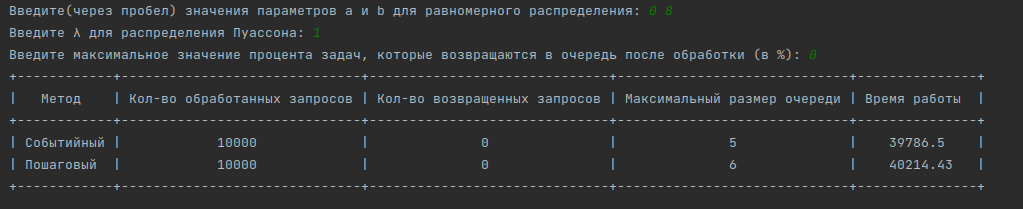
\includegraphics[scale=0.45]{pictures/1_0.png}}
\caption{Результат работы программы при отсутствии возвращения обработанных заявок в очередь}
\label{fig:1_0}
\end{figure}

\begin{figure}[H]
\center{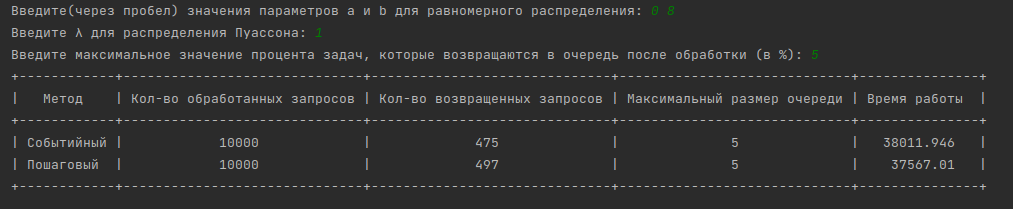
\includegraphics[scale=0.45]{pictures/1_5.png}}
\caption{Результат работы программы при возвращении в очередь не более 5\% обработанных заявок}
\label{fig:1_5}
\end{figure}

\begin{figure}[H]
\center{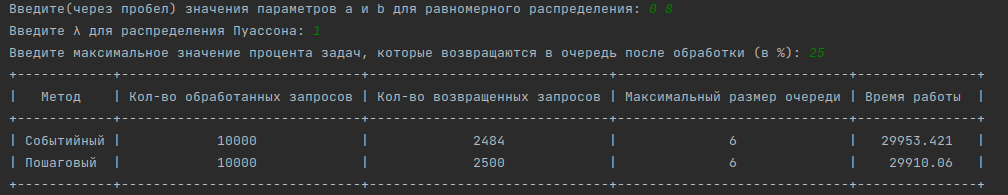
\includegraphics[scale=0.45]{pictures/1_25.png}}
\caption{Результат работы программы при возвращении в очередь не более 25\% обработанных заявок}
\label{fig:1_25}
\end{figure}

\begin{figure}[H]
\center{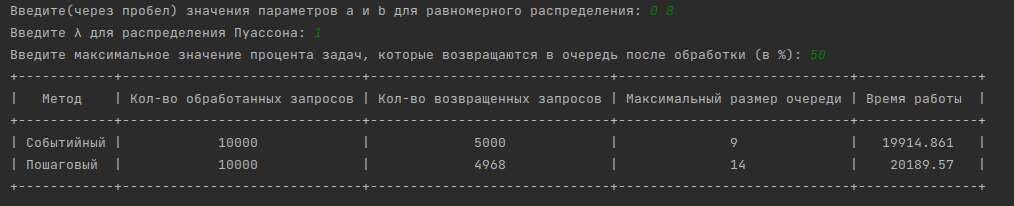
\includegraphics[scale=0.45]{pictures/1_50.png}}
\caption{Результат работы программы при возвращении в очередь не более 50\% обработанных заявок}
\label{fig:1_50}
\end{figure}

\begin{figure}[H]
\center{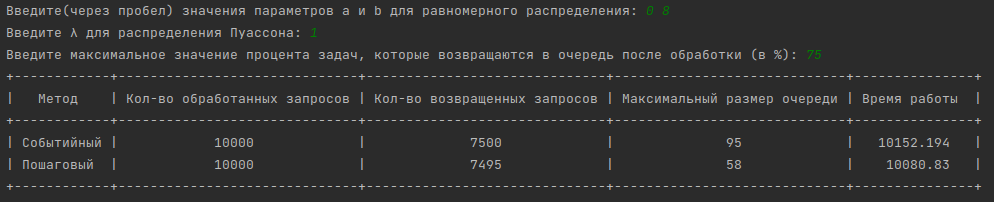
\includegraphics[scale=0.45]{pictures/1_75.png}}
\caption{Результат работы программы при возвращении в очередь не более 75\% обработанных заявок}
\label{fig:1_75}
\end{figure}

\begin{figure}[H]
\center{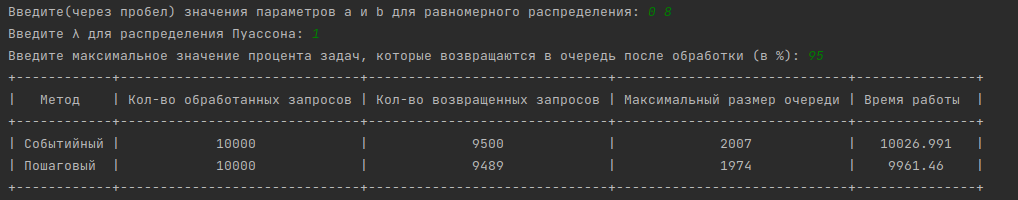
\includegraphics[scale=0.45]{pictures/1_95.png}}
\caption{Результат работы программы при возвращении в очередь не более 95\% обработанных заявок}
\label{fig:1_95}
\end{figure}

\begin{figure}[H]
\center{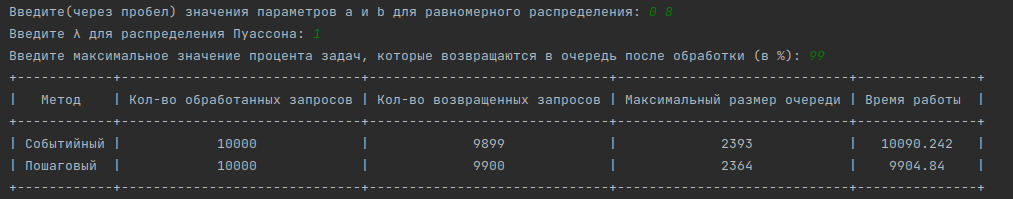
\includegraphics[scale=0.45]{pictures/1_99.png}}
\caption{Результат работы программы при возвращении в очередь не более 99\% обработанных заявок}
\label{fig:1_99}
\end{figure}

\begin{figure}[H]
\center{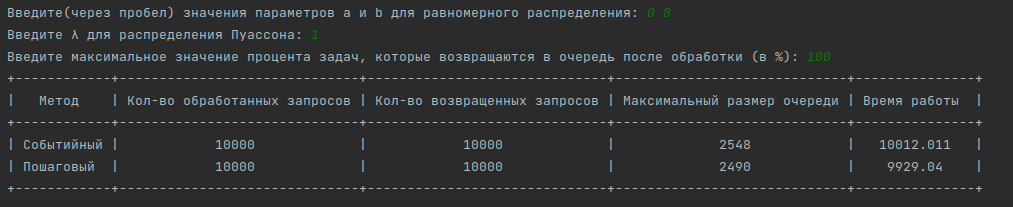
\includegraphics[scale=0.45]{pictures/1_100.png}}
\caption{Результат работы программы при возвращении в очередь всех обработанных заявок}
\label{fig:1_100}
\end{figure}

\subsection{$\lambda = 8$}
\begin{figure}[H]
\center{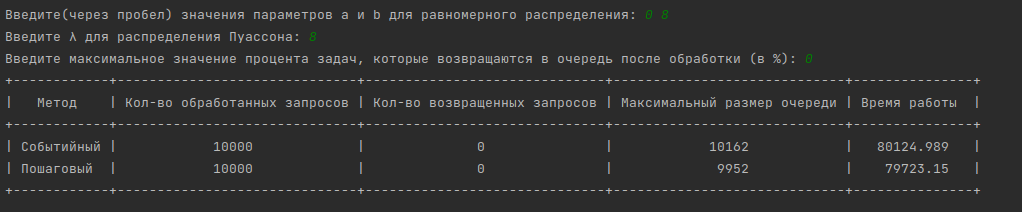
\includegraphics[scale=0.45]{pictures/8_0.png}}
\caption{Результат работы программы при отсутствии возвращения обработанных заявок в очередь}
\label{fig:8_0}
\end{figure}

\begin{figure}[H]
\center{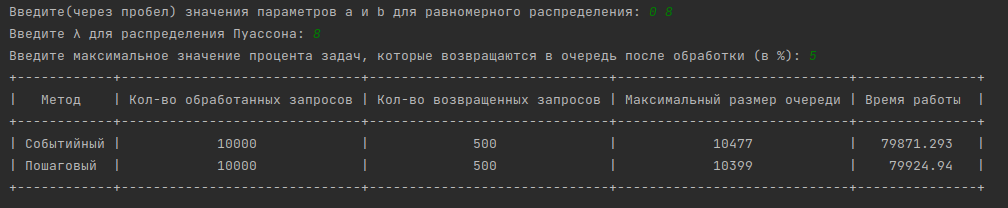
\includegraphics[scale=0.45]{pictures/8_5.png}}
\caption{Результат работы программы при возвращении в очередь не более 5\% обработанных заявок}
\label{fig:8_5}
\end{figure}

\begin{figure}[H]
\center{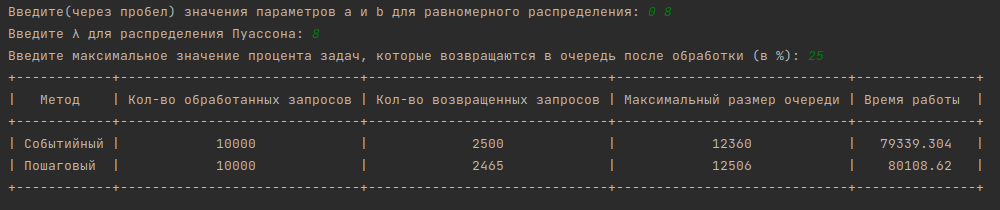
\includegraphics[scale=0.45]{pictures/8_25.png}}
\caption{Результат работы программы при возвращении в очередь не более 25\% обработанных заявок}
\label{fig:8_25}
\end{figure}

\begin{figure}[H]
\center{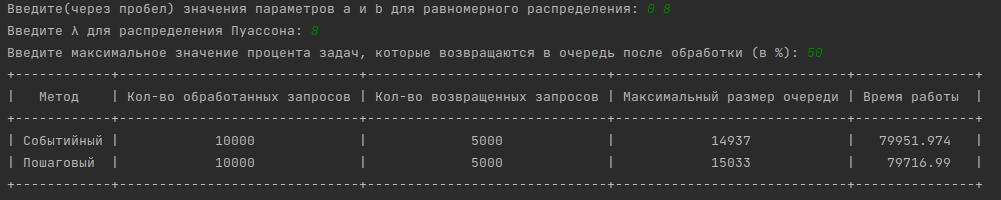
\includegraphics[scale=0.45]{pictures/8_50.png}}
\caption{Результат работы программы при возвращении в очередь не более 50\% обработанных заявок}
\label{fig:8_50}
\end{figure}

\begin{figure}[H]
\center{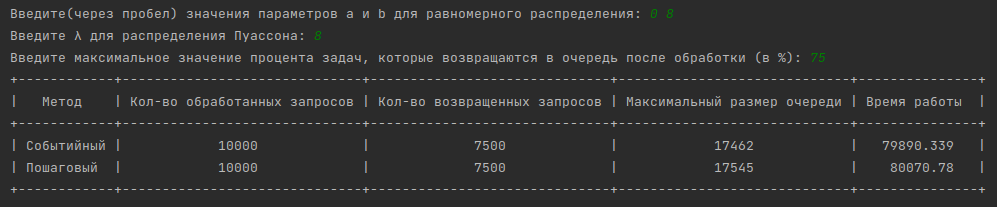
\includegraphics[scale=0.45]{pictures/8_75.png}}
\caption{Результат работы программы при возвращении в очередь не более 75\% обработанных заявок}
\label{fig:8_75}
\end{figure}

\begin{figure}[H]
\center{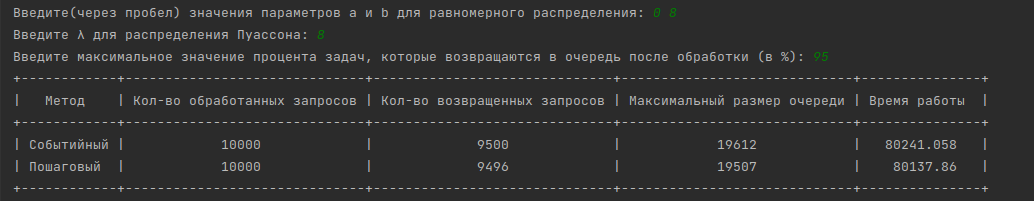
\includegraphics[scale=0.45]{pictures/8_95.png}}
\caption{Результат работы программы при возвращении в очередь не более 95\% обработанных заявок}
\label{fig:8_95}
\end{figure}

\begin{figure}[H]
\center{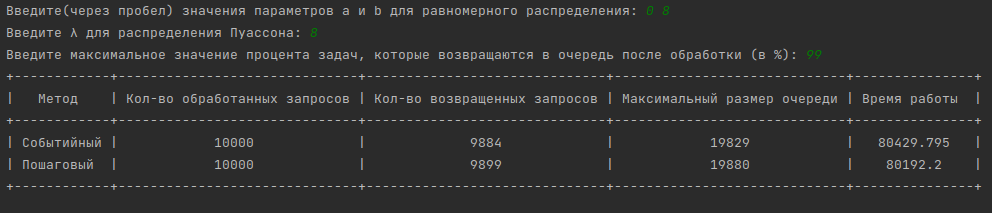
\includegraphics[scale=0.45]{pictures/8_99.png}}
\caption{Результат работы программы при возвращении в очередь не более 99\% обработанных заявок}
\label{fig:8_99}
\end{figure}

\begin{figure}[H]
\center{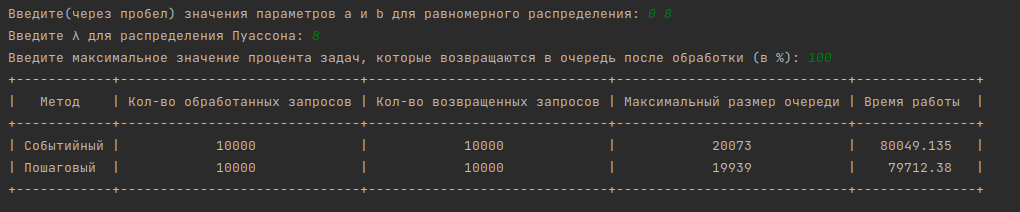
\includegraphics[scale=0.45]{pictures/8_100.png}}
\caption{Результат работы программы при возвращении в очередь всех обработанных заявок}
\label{fig:8_100}
\end{figure}

\section{Код программы}

Программа разработана в интегрированной среде разработки для языка программирования Python - PyCharm. 
В листинге 1 приведена реализация лабораторной работы.

\begin{lstlisting}[label=lst:list1]
from prettytable import PrettyTable
from scipy.stats import poisson, uniform
from numpy import random as numpy_random
import sys
COUNT = 10000
class Generator:
    def __init__(self, generator):
        self.generator = generator
        self.receivers = set()

    def add_receiver(self, receiver):
        self.receivers.add(receiver)

    def remove_receiver(self, receiver):
        try:
            self.receivers.remove(receiver)
        except KeyError:
            print("Ошибка!")
            sys.exit(0)

    def get_time(self):
        return self.generator.generate()

    def request(self):
        for receiver in self.receivers:
            receiver.receive_request()

class Processor(Generator):
    def __init__(self, generator, reenter_prob=0):
        super().__init__(generator)
        self.queue_size = 0
        self.max_queue_size = 0
        self.processed_requests = 0
        self.reentered_requests = 0
        self.reenter_prob = reenter_prob

    # Обработка запроса
    def process(self):
        if self.queue_size > 0:
            self.processed_requests += 1
            self.queue_size -= 1
            self.request()
            # Возвращение запроса в очередь при соблюдении условий вероятности
            if numpy_random.random_sample() <= self.reenter_prob and self.reentered_requests < self.reenter_prob * COUNT:
                self.reentered_requests += 1
                self.receive_request()

    # Добавление запроса в очередь
    def receive_request(self):
        self.queue_size += 1
        if self.queue_size > self.max_queue_size:
            self.max_queue_size = self.queue_size

class UniformDistribution:
    def __init__(self, a: float, b: float):
        self.a = a
        self.b = b
        self.scale = self.b - self.a

    def generate(self):
        return uniform.rvs(loc=self.a, scale=self.scale, size=1)[0]


class PoissonDistribution:
    def __init__(self, lmbda):
        self.lmbda = lmbda

    def generate(self):
        return poisson.rvs(self.lmbda, size=1)[0]


class Model:
    def __init__(self, uniform_a, uniform_b, lmbda, reenter_prop):
        self.generator = Generator(UniformDistribution(uniform_a, uniform_b))
        self.processor = Processor(PoissonDistribution(lmbda), reenter_prop)
        self.generator.add_receiver(self.processor)

    def event_based_system(self, request_count):
        generator = self.generator
        processor = self.processor

        gen_period = generator.get_time()
        proc_period = gen_period + processor.get_time()

        while processor.processed_requests < request_count:
            if gen_period <= proc_period:
                generator.request()
                gen_period += generator.get_time()
            if gen_period >= proc_period:
                processor.process()

                if processor.queue_size > 0:
                    proc_period += processor.get_time()
                else:
                    proc_period = gen_period + processor.get_time()

        return (processor.processed_requests, processor.reentered_requests,
                processor.max_queue_size, round(proc_period, 3))

    def time_based_modelling(self, request_count, dt):
        generator = self.generator
        processor = self.processor

        gen_period = generator.get_time()
        proc_period = gen_period
        current_time = 0
        while processor.processed_requests < request_count:
            if gen_period <= current_time:
                generator.request()
                gen_period += generator.get_time()
            if current_time >= proc_period:
                processor.process()
                if processor.queue_size > 0:
                    proc_period += processor.get_time()
                else:
                    proc_period = gen_period + processor.get_time()

            current_time += dt

        return (processor.processed_requests, processor.reentered_requests,
                processor.max_queue_size, round(current_time, 3))

if __name__ == '__main__':

    a, b = map(int, input("Введите(через пробел) значения параметров a и b для равномерного распределения: ").split())

    if a >= b:
        print("Параметр a должен быть меньше параметра b")
        sys.exit(0)

    lmbda = int(input("Введите лямбда для распределения Пуассона: "))

    if lmbda < 0:
        print("лямбда должна быть больше 0")
        sys.exit(0)

    repeat_probality = float(input("Введите максимальное значение процента задач, которые возвращаются в очередь после обработки (в %): "))
    if repeat_probality >= 0 and repeat_probality <= 100:
        repeat_probality = repeat_probality / 100
    else:
        print("Неверный ввод")
        sys.exit(0)

    total_tasks = COUNT
    step = 0.01

    model = Model(a, b, lmbda, repeat_probality)
    result1 = model.event_based_system(total_tasks)
    model2 = Model(a, b, lmbda, repeat_probality)
    result2 = model2.time_based_modelling(total_tasks, step)

    table = PrettyTable()
    table.add_column("Метод", ["Событийный", "Пошаговый"])
    table.add_column("Кол-во обработанных запросов", [result1[0], result2[0]])
    table.add_column("Кол-во возвращенных запросов", [result1[1], result2[1]])
    table.add_column("Максимальный размер очереди", [result1[2], result2[2]])
    table.add_column("Время работы ", [result1[3], result2[3]])
    print(table)
\end{lstlisting}
\end{document}